\section{Problem Formulation}
\label{sec:problemformulation}

% Modify related work


% Introduce the content of this section
The objective of the mesh network deployment is to minimize the number of 
deployed mesh nodes with the constraint of full coverage of the target area 
and connectivity to the Internet. In this section we first describe the 
the motivation of frequency agility, then we introduce 
the deployment constraints, which the QoS requirements of the vendors and clients.
Moreover, we discuss the frequency agility application impacts 
on a single access point and networks in dense and sparse areas.
Further, we formulate the deployment problem as a graph-theoretic model
with the QoS constraints an operational wireless mesh network must satisfy. 

\subsection{Motivation}
\label{subsec:motivation}
% Propagation -- Communication range
Wireless propagation is the behavior of the signal loss characteristics 
when wireless signals are transmitted through the wireless medium.
The strength of the received signal depends on both the line-of-sight
path (or lack thereof) and multiple other paths that result from 
reflection, diffraction, and scattering from obstacles
~\cite{andersen1995propagation}. The widely-used Friis equation 
characterizes the received signal power $P_r$ in terms of transmit 
power $P_t$, transmitter gain $G_t$, receiver gain $G_r$, wavelength
$\lambda$ of the carrier frequency, distance $R$ from transmitter to 
receiver, and path loss exponent $n$ according to~\cite{friis}:
\begin{equation}
\label{eq:friis}
P_r=P_t+G_t+G_r+10n \log_{10}\left( \frac{\lambda}{4\pi R}\right)
\end{equation}
Here, $n$ varies according to the aforementioned environmental 
factors with the value of two to five in typical outdoor 
settings~\cite{rappaport}. Through the propagation model, in 
the same environment with a constant path-loss exponent $n$, 
lower frequency white space bands offer not only more bandwidth, 
but also large communication range, which could potentially be 
used to reduce the number of access points. 

\begin{figure}
%\vspace{-0.0in}
\centering
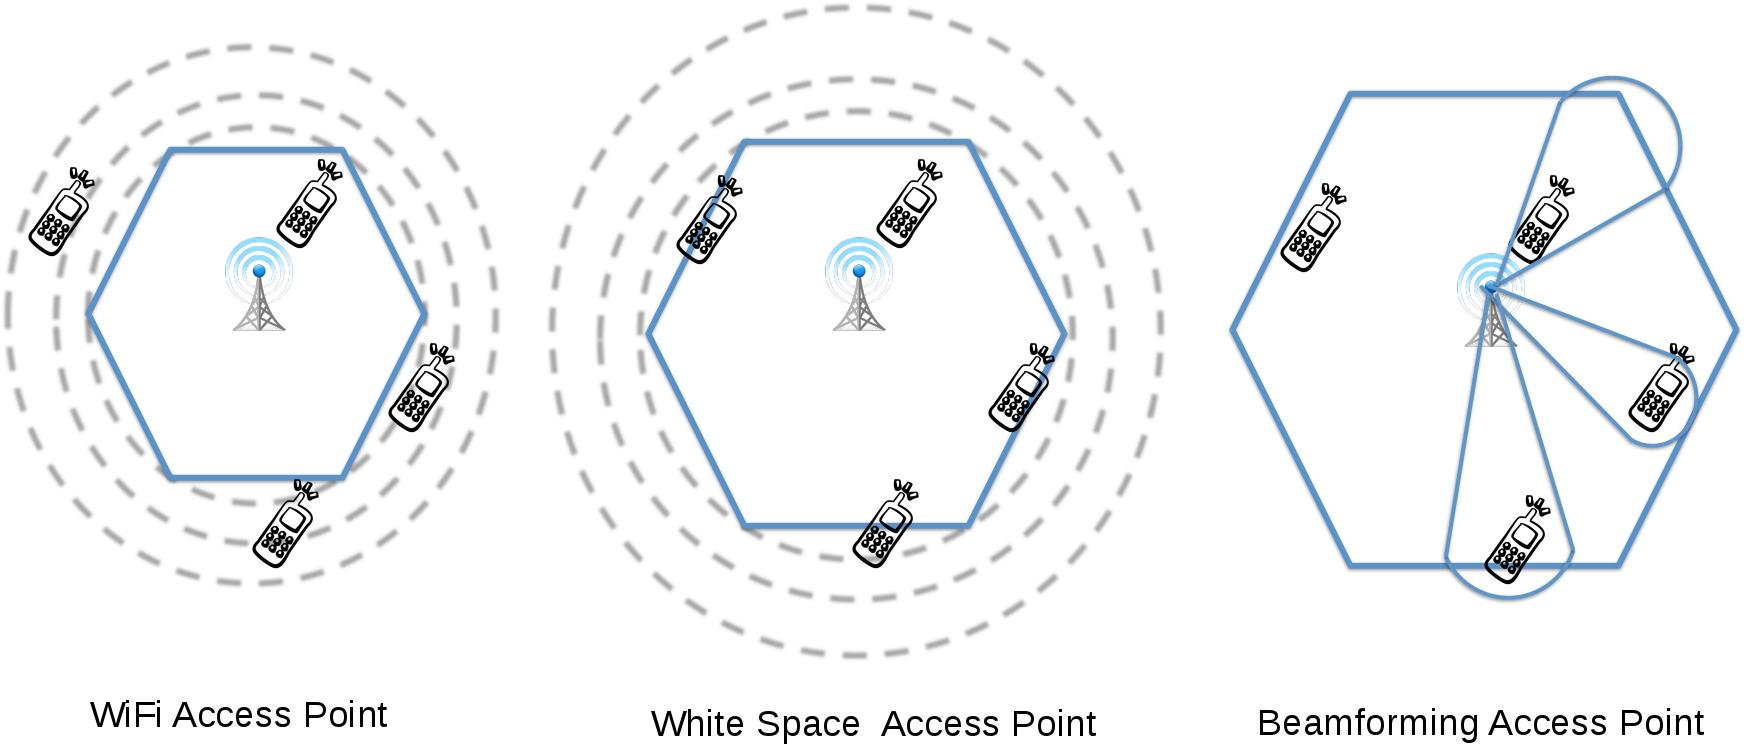
\includegraphics[width=84mm]{figures/com_range}
\vspace{-0.1in}
\caption{Communication Range of Access Points}                                                                 
\label{fig:aprange}
\vspace{-0.1in}
\end{figure}

Thus, access point with white space bands radios
could expand coverage region and increase a single access point capacity. 
However, at the same time, multiband radios application also increase the interference
range which reduce the re-use ability in the network. 
To further employ these technologies reducing the number of access points, 
the trade off between more coverage area and interference 
has to be optimized. In this work, we focus on this problem.
Before starting design a network, we introduce 
the network service constraints which are forced to 
be followed to satisfy the clients in the deployment. 

% Network Constraints
Typically, the deployment of wireless access networks is subject to coverage and capacity
constraints for a target area. Coverage is defined with respect to the ability of
clients to connect to access points within their service area.  We use a coverage
constraint ratio of $95\%$ in this work for a target area~\cite{robinson2010deploying}.
Capacity is defined with respect to the ability of a network to serve the traffic 
demand of clients.  Spatial reuse allows improved capacity, but increases the cost
of deploying a network by increasing the total number of access points required.
Hence, for densely populated areas the greatest level of spatial reuse 
is often desired which could be offered through an expensive new access point working 
in higher frequency.
In contrast, sparsely-populated rural areas have lower traffic demand per unit area. Thus, 
aggregating this demand with lower-frequency, white space bands 
could be highly effective in reducing the total number of access points required to achieve 
similar coverage and capacity constraints. 
Moreover, since less TV channels tend to be occupied in sparsely 
populated areas~\cite{msdatabase}, a larger number 
 of white space bands can be leveraged in these areas. 

% Lower frequency in sparse, higher frequency in dense.  
Under these constraints, the performance of the technology varies from dense 
populated area to sparse area. In dense populated area, more traffic demands
from unit area, which request more spacial reuse from higher frequency.
In \cite{cuimeasurement}, the channel occupancy varies with population density.
With a proper sweep schedule, more time spent for the dense part could 
compensate the capacity occupied by other devices. 
In sparse areas, few user generate low level traffic demand,
with less benefit for the service. Under these conditions, an access point
with lower frequency would be an affordable option. 
We will model these factors as parameters in a link graph 
and continue to analyze their influence in wireless network deployment.

\subsection{Model and Problem Formulation}
\label{subsec:problem}

% Assumptions of the network
As opposed to previous works such as~\cite{franklin2007node,robinson2010deploying
,si2010overview}, we focus on heterogeneous multiband access point selection 
for wireless access networks which jointly employ white space bands and WiFi bands.
Through white space and WiFi bands frequency agility, an access point performance could be
improve by the coverage area and throughput. 


We assume the service vendor has a limited number of spectrum resources and 
wireless radios have similar configuration, such as transmit power, 
gains. Each radio on an access point operates with a classic protocol 
model~\cite{gupta2000capacity}. Then we can further analyze the performance 
of access point under different traffic demand distribution according to the capacity 
and coverage constraint.

% Capacity constraint
A network deployment should ideally provide network capacity equal to the demand of the service 
area to maintain the capacity constraint. The demand of a service area could be calculated as the 
summation of individual demands all over the service area $D_a=\sum_{p\in P}D_p$. Since 
household demand for Internet has been previously characterized~\cite{rosston2011household}, 
$D_a$ could represent the population distribution $f$ and service area $k$ as 
$D_a=\sum_{f \in F,k \in K}\bar{D_p}*f*k$. 
The capacity constraint could be represented with access points set $M$ according to:
\begin{equation}
\label{eq:nlbound}
\sum_{m \in M}C_r^m \ge \sum_{f \in F,k \in K}\bar{D_p}*f*k
\end{equation}
% Coverage constraint
At the same time, the wireless network must additionally satisfy the coverage constraint in the service 
area where the access points provide connectivity for client devices. 
Generally, a coverage of $95\%$ is acceptable for wireless access networks~\cite{robinson2010deploying}.
The object of this work is to find the best possible number of access points so that the network has good 
connectivity and enough capacity to satisfy the traffic demands.

% Single  access point service analysis
Under the capacity and coverage constraints, the service area of an access point 
is limited by the propagation range and access point capacity. 
The radius of service area $r_s$ could be represented as:
\begin{equation}
\label{eq:servicearea}
r_s=min\{r_p,r_c\}
\end{equation}
$r_p$ represents the propagation range of the access point, $r_c$ is the capacity range of 
a radio in the access point. A simple example is when the traffic demand is distributed uniform in a circle, from 
Eq.~\ref{eq:nlbound} the capacity range $r_c$ could be noted as $r_c=\sqrt{k/\pi}$. 
Moreover, the propagation range and capacity rang could be determined by the environment, traffic distribution and
power control~\cite{robinson2010deploying}. 
These parameters could be pre-detected from existing measurements, census and public or private database.
When a target area is given, we could model the traffic demand, access points and
potential connectivity links as a graph according to the parameters from database.


% Problem
Thus, the target area with pre-defined parameters could be modeled as a connectivity graph with 
vertexes represented as the centralized traffic demand of a certain area and potential access points
locations. The edges note the links between the locations. 
Oppose to previous works,~\cite{robinson2010deploying,franklin2007node,tang2005interference,irwin2013resource}
we formulate the input connectivity graph as a graph $G = (V,E,F)$, where centralized
traffic demand, access points location candidates and links from a type of access point defined by
its frequency form a unified connectivity graph. 

The vertexes in the modeled input graph represent a set $C$ of  separated target area with traffic demands.
The set $C$ consists of physical coordinates representing target areas where client coverage is 
desired, analogous to the area to be covered in a geometric formulation and the traffic amount
need to be served.
And also the set of potential access points $M$ is a second part of the vertexes in the 
modeled graph. The potential locations of access points are assumed known through the 
infrastructure conditions.
The vertex set of the input connectivity graph is the union of potential access points
and centralized traffic demand locations as $V = C\cup M$.

The access points types set $F$ is defined by the working frequency band 
It is a set of different combination of frequency.
The set $E$ int the graph is the physical link under protocol model between two vertexes 
according to the access point type.

The output of the problem is expected to be an graph $G' = (V',E',F')$ which marks the access points
and chosen frequency. 
In the output graph, $V'$ includes the chosen access points set $M'$ and served traffic demand location
set $C'$. The set $F'$ tells the chosen access point type of each $M'$.
The connectivity and capacity constraints could be defined by the output graph $G'$, as shown 
in~\ref{eq:graph_coverage} and~\ref{eq:graph_capacity} 

\begin{equation}
\label{eq:graph_coverage}
\frac{\sum{Number\{C'\}}}{\sum{Number\{C\}}} \ge \theta_{coverage} 
\end{equation}
$\theta_{coverage}$ is the desired level of coverage for the target area. $C'$ is the 
served traffic demand location of the target area. 
 
\begin{equation}
\label{eq:graph_capacity}
C'_n \ge C_n\cdot \theta_{capacity}, C'_n \in C', C_n \in C
\end{equation}
$\theta_{capacity}$ is the percentage of satisfied traffic demand for the target area,
which also include the fairness request in the equation.

The output of the graph could be optimized in several aspects. From the view of vendors,
the number of access points would be the primary concern $Min{\{Number\{M'\}\}}$.
Through the vendors monthly income from flow charge, maximize the served traffic
demand would be the objective $Max{\{\sum{C'}\}}$. 

To optimize these parameters, 


